%!TEX root = ../main.tex

\section{Compton scattering}
\label{sec:compton-scattering}

Consider the scenario of a high-energy photon interacting with an unbound electron as
shown in \autoref{fig:compton-scattering}. To describe this process we choose a
coordinate frame where the electron is at rest with respect to us. In the experiments
to be presented in this report such a coordinate frame conveniently is the lab frame.
Furthermore, we employ natural units, $\epsilon_0=\hbar=c=1$. \\
From the conservation of energy and impluse a theoretical description of this process
can be constructed based on the inital and final energies of both particles.

\begin{align*}
E_{\gamma,i} + \underbrace{E_{e,i}}_{=0}\,&=\,E_{\gamma,f}+E_{e,f} \\
p_{\gamma,i} + \underbrace{p_{e,i}}_{=0}\,&=\,p_{\gamma,f}+p_{e,f} \\
\end{align*}

From the above relations an expression for the energy of the photon after interacting
with the electron can be obtained as lined out in \cite{Sch17}. The expression reads

\begin{equation}
\label{eq:photon-energy}
E_{\gamma,f}=\frac{E_{\gamma,i}}{1+\frac{E_{\gamma,i}}{m_e}(1-\cos\theta)},
\end{equation}

where $\theta$ defines the angle spanned between the incident photon and its path
post scattering. It follows that the electron gains energy from the interaction.

\begin{equation}
\label{eq:electron-energy}
E_{e,f}=E_{\gamma,i}-E_{\gamma,f}=E_{\gamma,f}\cdot\frac{E_{\gamma,i}}{m_e}\cdot(1-\cos\theta).
\end{equation}

The measureable change in the photons wavelength $\lambda=\frac{hc}{E_{\gamma}}$
due to the interaction is called the \textbf{Compton effect}. The underlaying elastic
scattering of photons and unbound electrons is consequently labelled \textbf{Compton
scattering}. Alongside Photoionisation and Pair production it represents one of the
important processes by which electromagnetic radiation interacts with matter.

The physical characteristics of Compton scattering, namely its cross section and
the resulting distribution of electron energies will be discused in the following
\autoref{sec:compton-cross-section} and \autoref{sec:compton-spectrum}.

\begin{figure}
\centering
\begin{subfigure}[h]{0.5\linewidth}
\centering
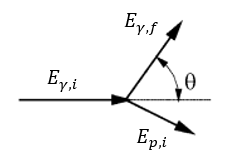
\includegraphics[height=4.2cm]{fig/compton-scattering.png}
\caption{\textbf{Scattering kinematics}\label{fig:compton-scattering}}
\end{subfigure}%
\begin{subfigure}[h]{0.5\linewidth}
\centering
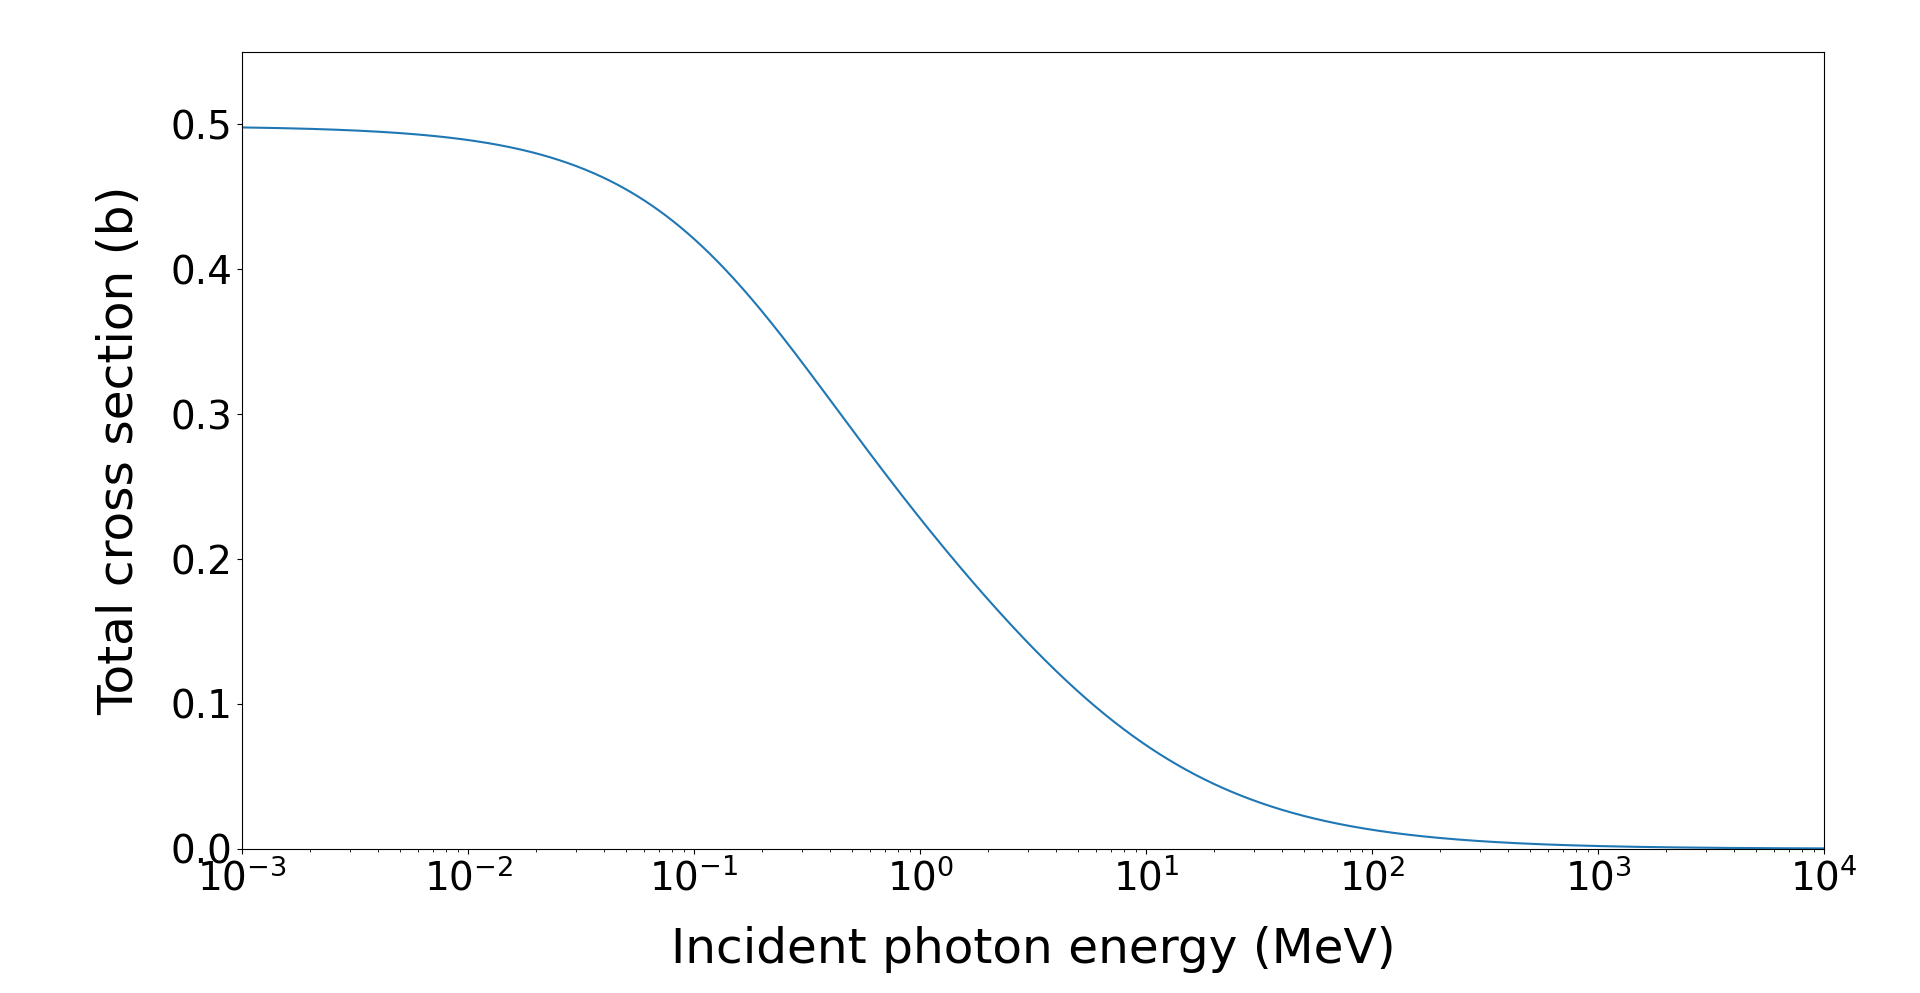
\includegraphics[height=4.2cm]{fig/compton-cross-section.png}
\caption{\textbf{Total cross section}\label{fig:compton-cross-section}}
\end{subfigure}%
\caption*{(a) A high energy photon scatters off a free electron at
rest. The defining variables to describe this process are given by $E_{\gamma,i}$
and $\theta$. Figure adapted with changes from \cite{Sch17}.
(b) The total cross section for compton scatter as a function of the incident photon 
energy. Roughly constant for low-energy photons, the total cross section drops off
for higher energies.}
\end{figure}

\newpage
